\documentclass[../review_1.tex]{subfiles}
\graphicspath{{\subfix{../img/}}}
\begin{document}

\chapter{Anforderungsanalyse}\thispagestyle{fancy} %Kopf- und Fußzeile an
\vspace{-1.5cm}
\begin{figure}[h]
    \centering
    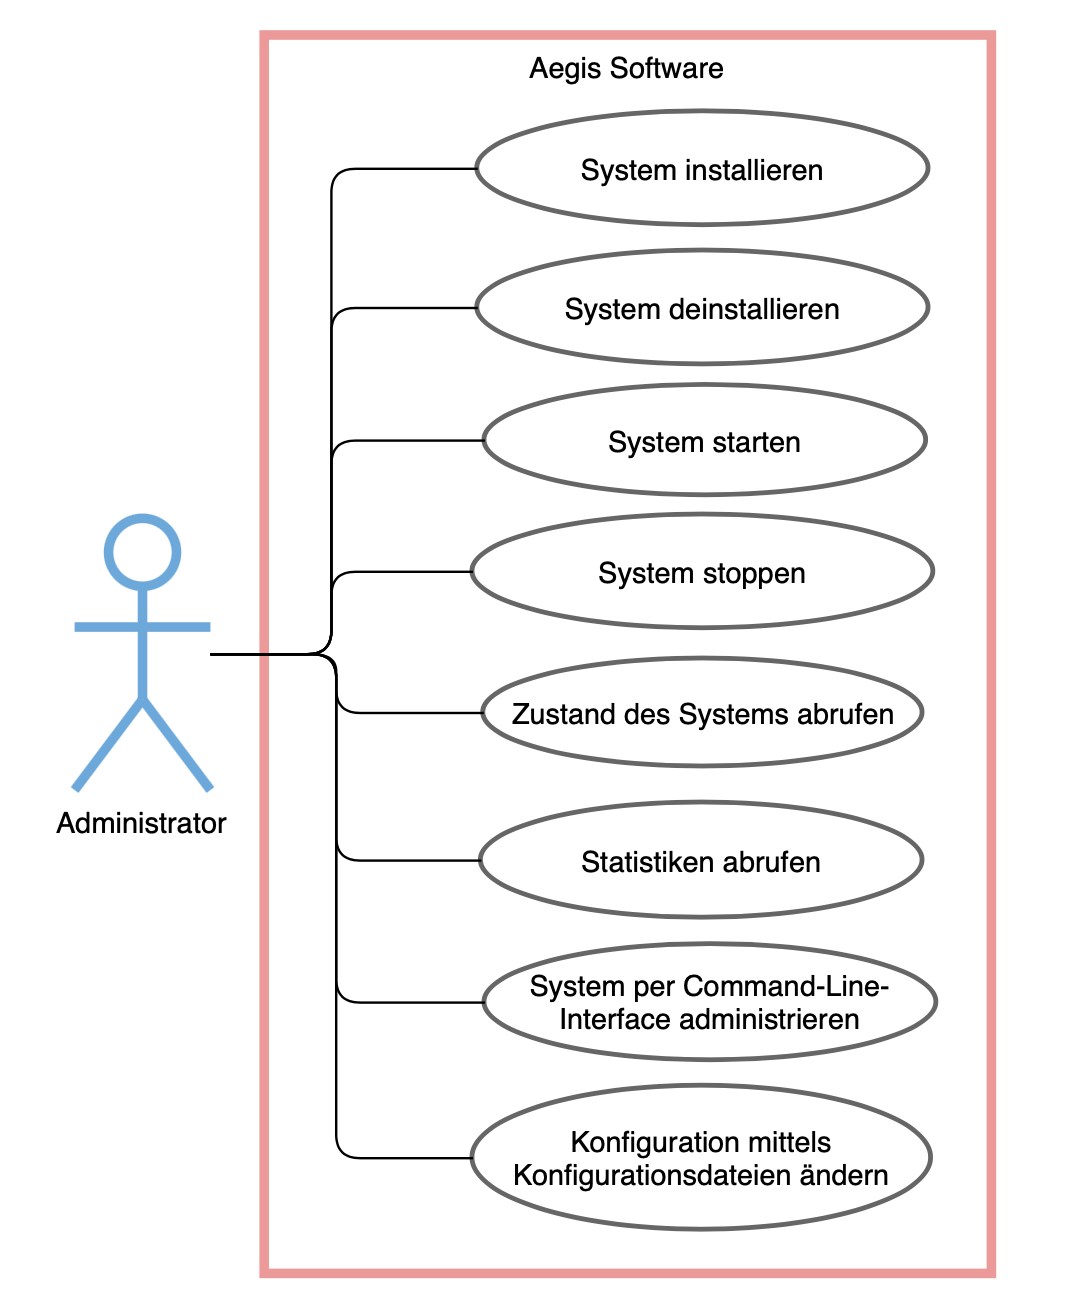
\includegraphics[height = 8cm]{usecase1.png}
    \caption{UML-konformes Use-Case-Diagramm}
    \label{usecase1}
\end{figure}
\noindent  Es wurde sich dafür entschieden, auch Akteure in das unten stehende Use-Case-Diagramm (siehe Abb. \ref{usecase2}) aufzunehmen, die nach den UML-Standards nicht in einem Use-Case-Diagramm (siehe Abbi. \ref{usecase1}) vorkommen.\\
Dadurch können auch Use-Cases modellieren werden, die über das Installieren und die grundlegenden administrativen Aufgaben hinausgehen.\\
So agiert beispielsweise der Angreifer in Abb. \ref{usecase1} nicht mit dem System. Jedoch ist er für das Verständnis, welche Schutzmechanismen ergriffen werden müssen, unerlässlich. Deshalb ist er in Abb. \ref{usecase2} hinzugekommen.\\
Der normale Nutzer soll möglichst wenig bis gar nichts vom Abwehrsystem mitbekommen, weswegen er nur mit wenigen Anwendungsfällen in Beziehung steht. \\
Somit ist dieses Anwendungsfalldiagramm  ein Beispiel dafür, dass die Diagramme in diesem Projekt eine Sonderrolle einnehmen.
\begin{figure}[ht]
    \centering
    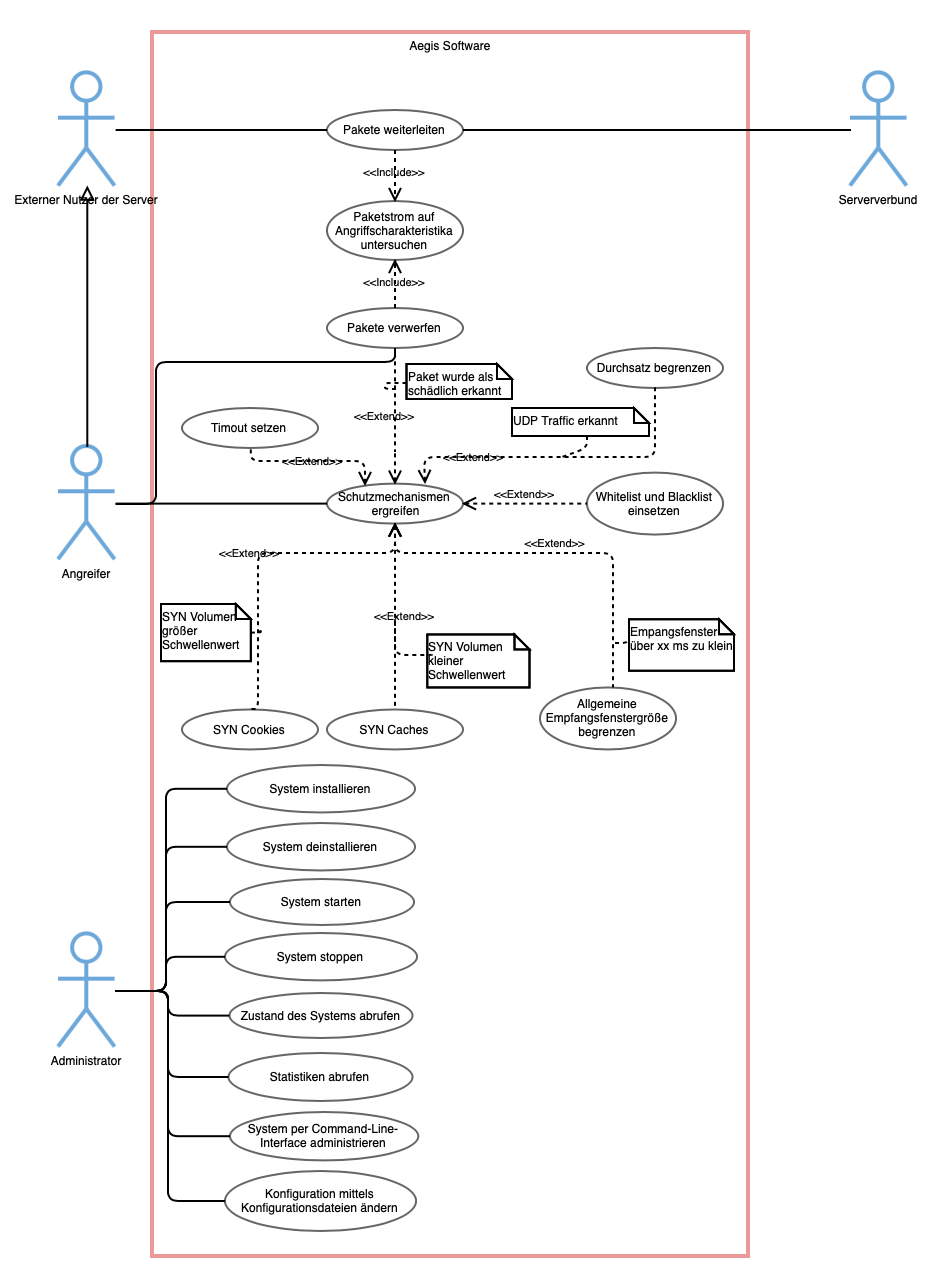
\includegraphics[width=13cm]{usecase2.png}
    \caption{nicht UML-konformes Use-Case-Diagramm}
    \label{usecase2}
\end{figure}

\end{document}
